\documentclass[a4paper,10pt]{report}
\usepackage[utf8x]{inputenc}
\usepackage{graphicx}
\usepackage[brazil]{babel}
\usepackage{hyperref}
\usepackage{html,makeidx}

%specific to HTML output
%\htmltitle{Fundamentos de Computação Gráfica - INF2608}
%\htmladdress{robertogerson@telemidia.puc-rio.br}
%\htmlcss{http://www.w3.org/StyleSheets/Core/Modernist}

% Title Page
\title{Fundamentos de Computação Gráfica - INF2608}
\author{Roberto Gerson de Albuquerque Azevedo}

\begin{document}
\maketitle

\begin{abstract}
Este documento apresenta os trabalhos desenvolvidos, bem como suas bases
teóricas, no escopo da disciplina \htmladdnormallink{Fundamentos
de Computação Gráfica (FCG) -
INF2608}{http://www.tecgraf.puc-rio.br/~mgattass/fcg/fcg.html}, cursada
durante o Doutorado em Informática pela PUC-Rio. A disciplina de FCG é subdivida
em três partes principais: Luz e Cor, Imagem e 3D. Para cada uma dessas partes é
sugerido o desenvolvimento de um projeto. As seções a seguir detalham cada um
desses projetos.
\end{abstract}

\chapter{Luz e Cor}
\par
Sendo a Computação Gráfica (CG) a área da computação destinada ao estudo de
modelos e algoritmos para o processamento de imagens digitais, o estudo da cor é
um dos seus fundamentos. A cor é uma sensação que os seres humanos têm em
resposta à luz incidente em nossos olhos. Sendo assim, o estudo da cor está
diretamente relacionado com o estudo da luz.

\par
Com o objetivo de melhor entender como nós percebemos as cores e a importância
de se definir um sistema no qual seja simples representá-las, permitindo, por
exemplo, reproduzí-las em ambientes virtuais, o seguinte trabalho foi proposto:

\section{Enunciado do Trabalho}
\par
Um dos padrões de cor mais difundidos é o Macbeth Color Checker
ilustrado na figura abaixo.

\begin{figure}[!htb]
     \centering
     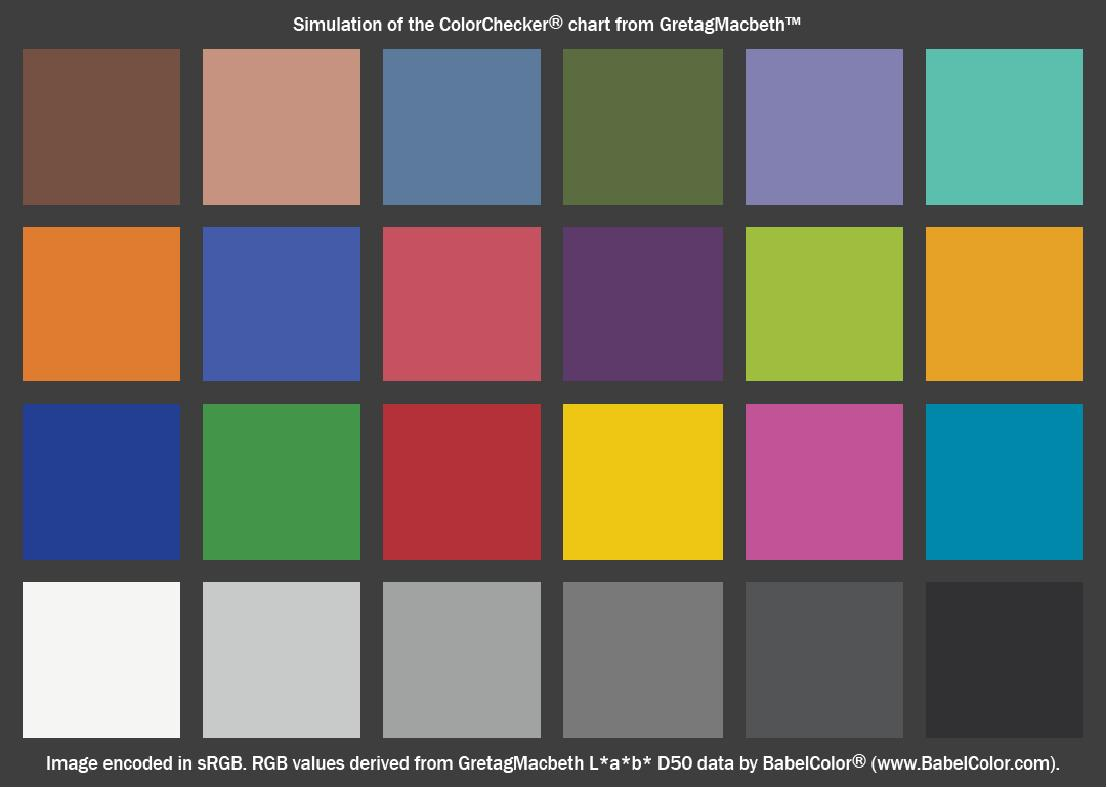
\includegraphics[scale=0.4]{img/colorChecker.jpg}
     \caption{Macbeth Color Checker. Fonte: URL}
     \label{Label de referência para a imagem}
\end{figure}

\par
Considere as amostras armazenadas por linha da esquerda para a direita de cima
para baixo.  Desta foram na última linha temos os tons de cinza e as quatro
primeiras cores são: pele escura(dark skin), pele clara(light skin), azul céu
(blue sky) e folhagem (foliage), respectivamente.  

\par
O trabalho de cor deste ano consiste em:
\newcounter{qcounter}
\begin{list}{\arabic{qcounter}:~}{\usecounter{qcounter}}
\item A partir do espectro fornecido calcular as componentes CIEXYZ,
CIExyY, CIELuv, CIELab e sRGB destas quatro primeiras amostras.
\item Somar os espectros da pele clara com o céu azul e calcular, a partir deste
novo espectro as componentes CIEXYZ, CIExyY, CIELuv, CIELab e sRGB.
\item Verificar a linearidade destes sistemas.
\end{list}

\section{Conceitos Básicos}
\par
Antes de discutirmos como se deu a implementação do trabalho, é importante
definirmos alguns conceitos básicos e como se dá o processo de percepção e
adição de cores, os quais serão úteis para as discussões seguintes.

\subsection{Luz}
\par
Da Física, sabemos que a luz tem um comportamento dual, as vezes se comportando
como um feixe de partículas e outras como uma onda. Aqui estamos muito mais
interessados em seu comportamento como onda, sendo que geralmente a
caracterizamos por meio de seu comprimento de onda ou frequência. Cabe
ressaltar, entretanto, que a luz vísivel é apenas uma pequena parte das
chamadas onda eletromagnéticas (indo de aproximada 380nm até 780nm).

\begin{figure}[!htb]
     \centering
     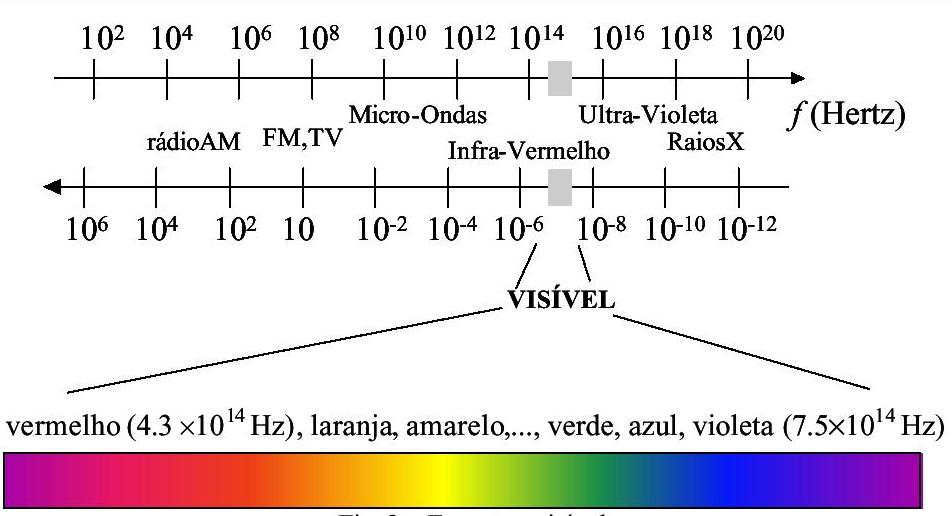
\includegraphics[scale=0.4]{img/visible_spectrum.jpg}
     \caption{Faixa de espectro visível. Fonte:
\htmladdnormallink{Gattas, Marcelo}{
http://www.tecgraf.puc-rio.br/~mgattass/cg/pdf/02_CorPPT.pdf}}
     \label{fig:visible_spectrum}
\end{figure}

\par
Para os nossos propósitos, a luz é descrita por meio de uma curva de
distribuição espectral sobre o espectro visível . Um tipo específico de luz
emite diferentes quantidades de energia em cada parte do espectro visível. A
Figura \ref{fig:visible_spectrum} apresenta o exemplo do espectro de uma luz do
dia.

\begin{figure}[!htb]
     \centering
     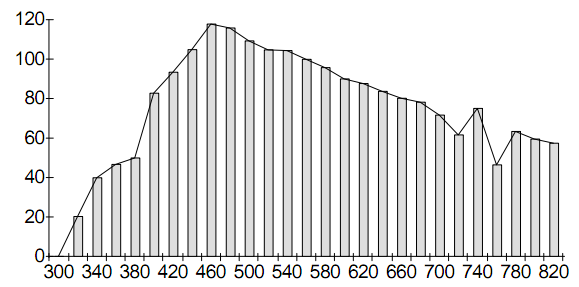
\includegraphics[scale=0.6]{img/spectrum_light.png}
     \caption{Espectro da Luz do dia. Fonte:
\htmladdnormallink{DiCosola, Michael}{
http://www.xrite.com/documents/apps/public/whitepapers/Ca00002a.pdf}}
     \label{fig:visible_spectrum}
\end{figure}

\par
Cada comprimento de onda presente no espectro visível é associado a uma cor.
Quando temos um espectro que emite energia em apenas um dos comprimentos de
onda, o chamamos de espectro puro. Consequentemente, as cores associadas à
este tipo de espectro são chamadas de cores de espectro puro (ou 100\%
saturadas).

\subsection{Fontes de Luz e Iluminantes}
\par
A luz é produzida por uma fonte de luz. Adicionalmente, também é importante
definirmos a diferença de uma fonte de luz para um iluminante.
Uma fonte de luz é algo realmente físico, que existe e pode ser ligada ou
desligada para iluminar algo. Por outro lado, um iluminante é uma luz que foi
definida apenas pela sua distribuição espectral, mas não necessariamente existe.
Assim, se, através de experimentos definirmos a distribuição espectral de uma
fonte de luz sobre um branco, nós definimos um iluminante. Essa diferença é
importante pois estamos muito mais interessados nos iluminantes, os quais
existindo ou não, podemos estudar numericamente, como um determinado será
visualizado quando iluminado por ele.

\par
Exitem vários iluminantes que são padronizados. As Figuras a seguir apresentam
o espectro de dois desses iluminantes, D50 e D65, que serão utilizados na
implementação deste trabalho.

\begin{figure}[!htb]
     \centering
     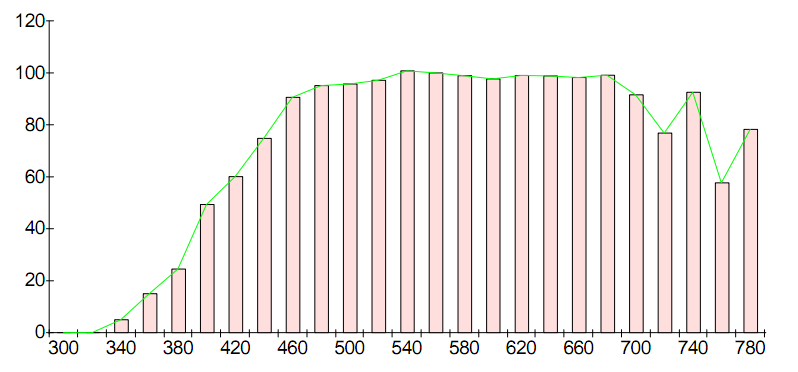
\includegraphics[scale=0.6]{img/illuminant_d50.png}
     \caption{Espectro do iluminante D50. Fonte:
\htmladdnormallink{DiCosola, Michael}{
http://www.xrite.com/documents/apps/public/whitepapers/Ca00002a.pdf}}
     \label{fig:illuminant_d50}
\end{figure}

\begin{figure}[!htb]
     \centering
     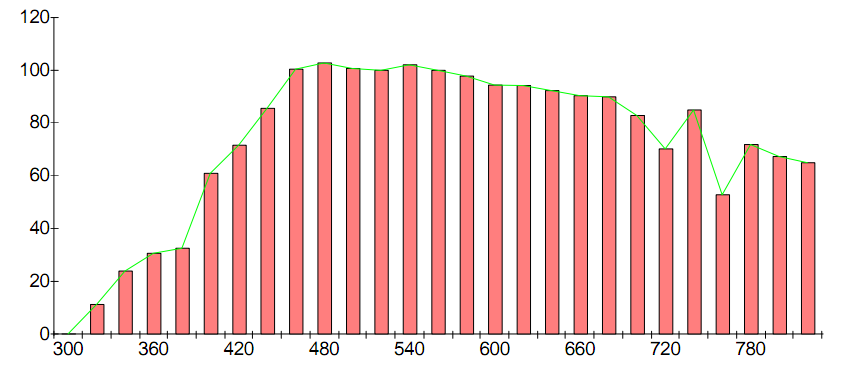
\includegraphics[scale=0.6]{img/illuminant_d65.png}
     \caption{Espectro do Iluminante D65. Fonte:
\htmladdnormallink{DiCosola, Michael}{
http://www.xrite.com/documents/apps/public/whitepapers/Ca00002a.pdf}}
     \label{fig:illuminant_d65}
\end{figure}

\subsection{Espectros de cores}
\par
A cor de um objeto nada mais é do que o espectro resultante de todas as
interações da luz com ele e que ele emite. É fácil perceber que ao ser iluminado
por fontes de luz diferentes um mesmo objeto pode ter cores diferentes. Isso
porque a própria fonte de luz também tem uma cor. Isso fica claro quando a
definimos como um iluminante, pois sua distribuição espectral define a "cor" do
iluminante.

\par
A superfície de um objeto pode refletir de forma diferente diferentes
comprimentos de onda. Sendo assim, também é possível caracterizar a
reflectância de um objeto por meio de um gráfico onde, para cada comprimento de
onda, temos a porcentagem de energia que essa superfície reflete. De posse
desses dois dados podemos então calcular qual o espectro resultante, e
consequentemente a cor, que esse objeto terá quando iluminado com um
determinado iluminante. A Figura a seguir mostra esquematicamente este processo.

\begin{figure}[!htb]
     \centering
     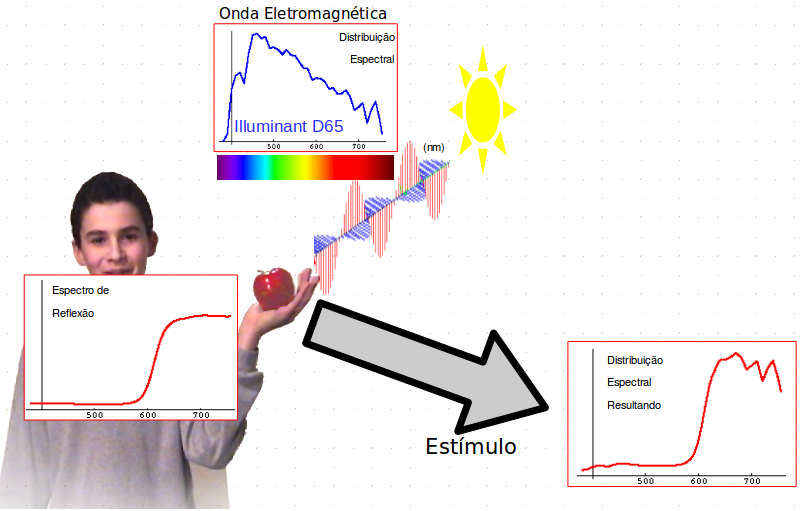
\includegraphics[scale=0.9]{img/spectrum_reflection.png}
     \caption{Espectro resultante da reflexão da luz de um iluminante em
um objeto. Fonte: Adaptado de \htmladdnormallink{Gattas, Marcelo}
{http://www.tecgraf.puc-rio.br/~mgattass/cg/pdf/02_CorPPT.pdf}.}
     \label{fig:spectrum_reflection}
\end{figure}

\subsection{Observador CIE padrão}
\par
Contudo, nem tudo é tão simples como parece. A percepção de cor é um fenômeno
muito mais contextual do que pode parecer a primeira vista. Por exemplo, uma
mesma cor com diferentes planos de fundo tendem a parecer diferente para nós.
Além disso, a cor também é dependente do tamanho dos objetos que estamos
visualizando. Tudo isso torna o processo de representação e reprodução de cor
muito mais complexo do que pode parecer.

\par
Mesmo assim, existe muita evidência de que uma teoria baseada em três estímulos
de cor é bastante útil para muitas aplicações práticas. De acordo com a teoria
da tri-cromaticidade, um observador pode perceber uma cor como uma mistura
aditiva de três estímulos primários.

\par
Baseado nesta teoria e em testes empíricos, onde são requisitados para
observadores enunciarem quais as cores que estão vendo a partir de uma mistura
de três cores primarias, o \htmladdnormallink{International
Commission on Illumination (CIE)}{http://cie.co.at} definiu, em 1931,
a curva da Figura abaixo. Essa curva apresenta resultados empíricos para
observadores com um campo de visão de 2 graus. Em 1964, uma nova curva, um
pouco diferente dessa, foi desenvolvida com observadores contendo 10 graus.

\begin{figure}[!htb]
     \centering
     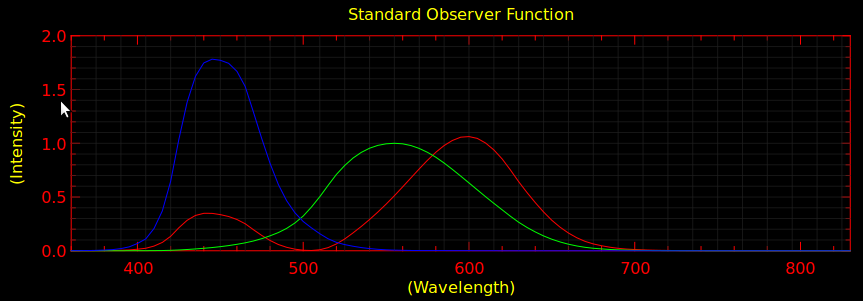
\includegraphics[scale=0.8]{img/cie_std_observer.png}
     \caption{Observador Padrão CIE.}
     \label{fig:standard_observer}
\end{figure}

\par
Esse gráfico mostra a quantidade relativa das três cores primárias
(aproximadamente vermelho, azul e verde) que deve ser fornecida para que um
observador regular possa distiguir uma unidade de luz comprimento de onda. Como
é possível observar pelo gráfico, a sensibilidade das células fotoceptoras
(os cones e bastonetes) em nossos olhos são diferentes para cada comprimento de
onda, de tal forma que a energia em alguns comprimentos de onda precisam ser
maior para percebemos alguma diferença.

\par
Sendo assim, a Figura \ref{fig:spectrum_reflection} na verdade também tem que
levar em consideração a sensibilidade do olho humano, como mostra a Figura a
seguir.

\begin{figure}[!htb]
     \centering
     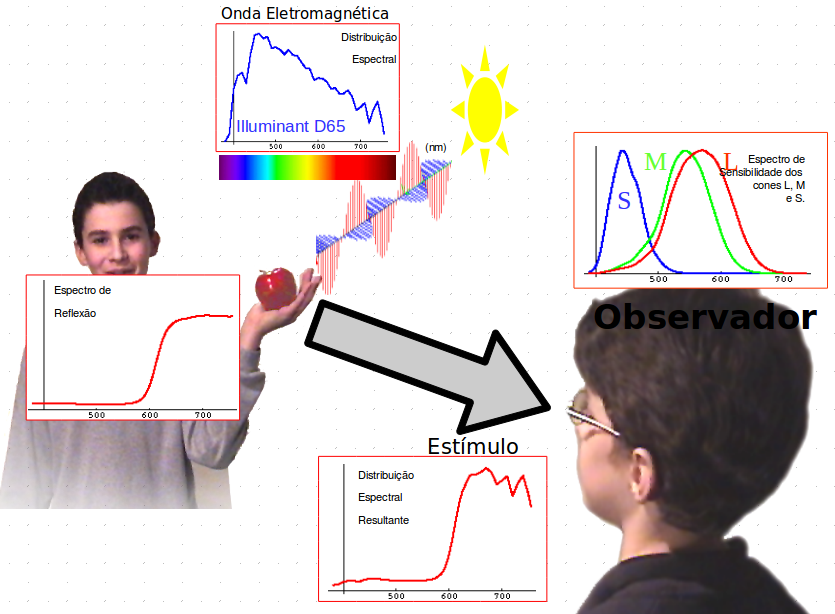
\includegraphics[scale=0.9]{img/what_is_color.png}
     \caption{Processo de formação de cor como resultado da interação de um
espectro de um iluminante e o espectro de reflexão de um objeto. Fonte:
Adaptado de \htmladdnormallink{Gattas, Marcelo}
{http://www.tecgraf.puc-rio.br/~mgattass/cg/pdf/02_CorPPT.pdf}.}
     \label{fig:what_is_color}
\end{figure}

\subsection{Processo aditivo de formação de cor}
\par
Diferente da percepção que temos do som por exemplo, ao adicionarmos duas cores,
o olho humano não consegue diferenciar componentes e sim uma nova cor
resultante. Neste trabalho, em especial, estamos interessado em analisar o que
acontece quando somamos duas cores nos diferentes espaços de cores que existem,
e que serão detalhados mais a frente.

\par
Antes de analisarmos o que acontece com os diferentes espaços de cor,
entretanto, já temos capacidade de discutir o que acontece quando, por exemplo,
quando iluminamos uma mesma região com duas fontes de luz diferente. Como
resultado, teremos um espectro resultante que é a soma dos dois espectros
individuais, conforme mostra a figura abaixo. Essa é uma das formas de criarmos
novas cores a partir de outras.

\begin{figure}[!htb]
     \centering
     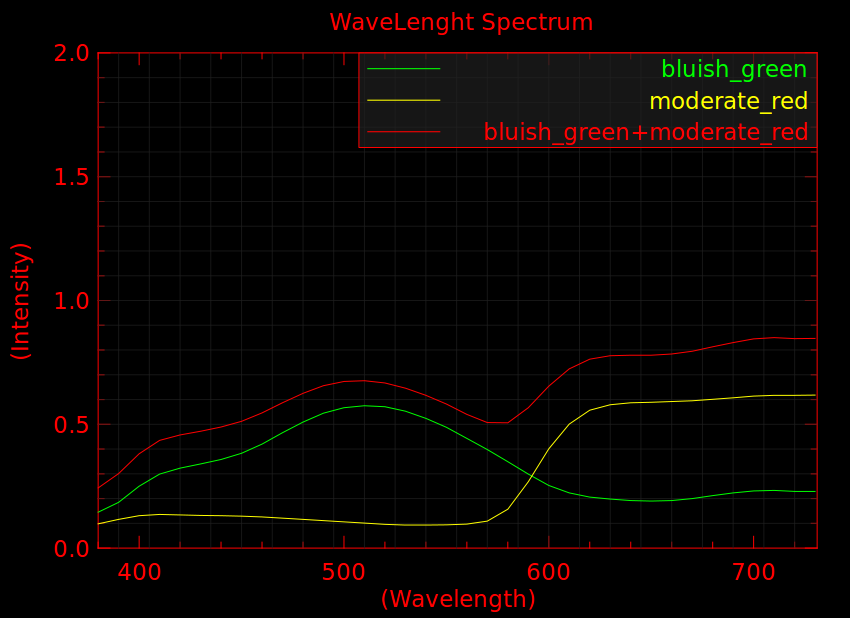
\includegraphics[scale=0.6]{img/color_addition.png}
     \caption{Adição de espectro de cores gerada a partir do aplicativo
desenvolvido por este trabalho.}
     \label{fig:color_addition}
\end{figure}

\section{Implementação}
Para apoiar a análise da linearidade dos espaços de cor, que serão detalhados
na seção a seguir, um aplicativo foi desenvolvido em C/C++. Esse aplicativo
utiliza o \htmladdnormallink{Qt}{http://qt.nokia.com}, para permitir a
independência de
sistema operacional, e a biblioteca
\htmladdnormallink{plplot}{http://plplot.sourceforge.net}, para desenho dos
gráficos.

\par
No aplicativo desenvolvido é possível, a partir da descrição dos espectros de
cores informado como entrada, selecionar duas cores. A partir dos espectros
informados essas cores são convertidas para os espaços XYZ, xyZ, L*u*v*,
L*a*b* e sRGB. A cor resultando da adição das duas cores selecionadas também é
convertida para cada um desses espaços de cores.

\subsection{Metodologia}
\par
Como entrada, o programa recebe: a descrição do observador padrão CIE, o
espectro de reflectância de cada cor Macbeth Color Checker e a
descrição dos iluminantes que podem ser utilizados.

\par
O cálculo de como as diversas cores do Macbeth Color Checker irão
aparecer sobre os diversos iluminantes, bem como o resultado de como a soma
destas duas cores também aparecerá é realizada baseando-se no que expõe
\htmladdnormallink{Lindbloom, Bruce}
{http://www.brucelindbloom.com/Eqn_Spect_to_XYZ.html}.

\par
A princípio, os três estímulos do espaço XYZ são calculados, por meio das
fórmulas a seguir:

\begin{equation}\label{eq:XYZfromSpectrum_X}
X=\frac{1}{N}.\sum{xbar_i.S_i.I_i}
\end{equation}

\begin{equation}\label{eq:XYZfromSpectrum_Y}
Y=\frac{1}{N}.\sum{ybar_i.S_i.I_i}
\end{equation}

\begin{equation}\label{eq:XYZfromSpectrum_Z}
Z=\frac{1}{N}.\sum{zbar_i.S_i.I_i}
\end{equation}

\begin{equation}\label{eq:XYZfromSpectrum_N}
N=\frac{1}{N}.\sum{ybar_i.I_i}
\end{equation}

\par
De posse desses estímulos é possível transfomá-los nas representações dos
espaços de cor xyZ, L*u*v*, L*a*b e sRGB. As fórmulas para cada um destes
espaços são apresentadas na Seção \ref{sec:analise_espacos_de_cor};

\par
A soma das duas cores é realizada ainda no espectro de reflexão, mas é fácil
perceber que o mesmo resultado seria alcançado se a soma fosse calculada apenas
após o cálculo do espectro resultante em cada uma das cores.

\subsection{Screenshots}
\par
Esta seção apresenta alguns screenshots do programa desenvolvido. No lado
esquerdo da tela inicial, apresentada a abaixo, o usuário pode escolher um par
de cores, bem como qual o iluminante que deseja utilizar.

\begin{figure}[!htb]
     \centering
     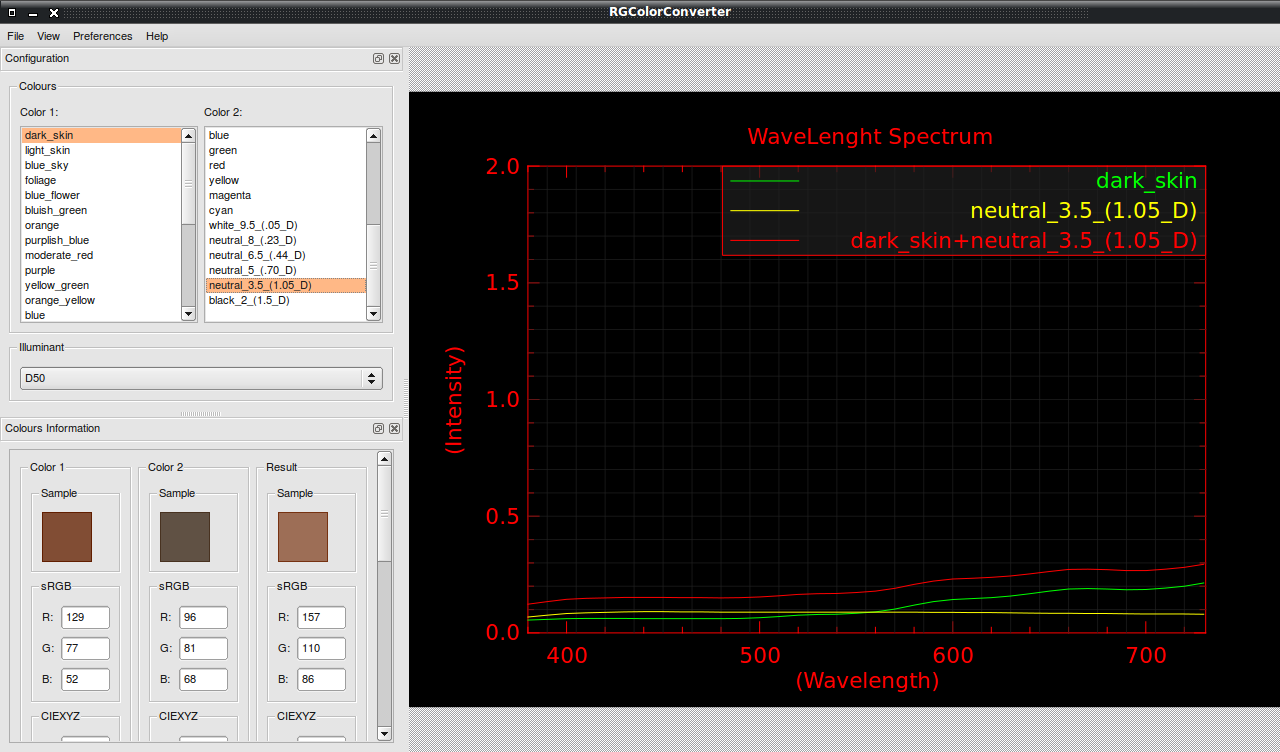
\includegraphics[scale=0.6]{img/screenshot_RGColorConverter.png}
     \caption{Screenshot do espectro da soma duas cores}
     \label{fig:screenshot_01}
\end{figure}

\par
Na aba "View", o usuário pode escolher quais os gráficos que ele deseja
que seja desenhados. Além dos gráficos dos espectros de reflexão, das cores
iniciais e da soma, também é possível escolher visualizar o gráfico do
observador padrão CIE e do iluminante, ambos carregados a partir arquivos de
dados. Sendo assim, é possível, por exemplo, facilmente trocar entre os dados
para o observador de 2 graus ou 10 graus.

\par
Adicionalmente, também é possível apresentar os sistemas de coordenadas de cada
um dos espaços de cor apresentados e os pontos onde cada uma das cores (as
escolhidas e a soma delas). Isso é útil para que possamos estudar a linearidade
de cada um desses sistemas.

\begin{figure}[!htb]
     \centering
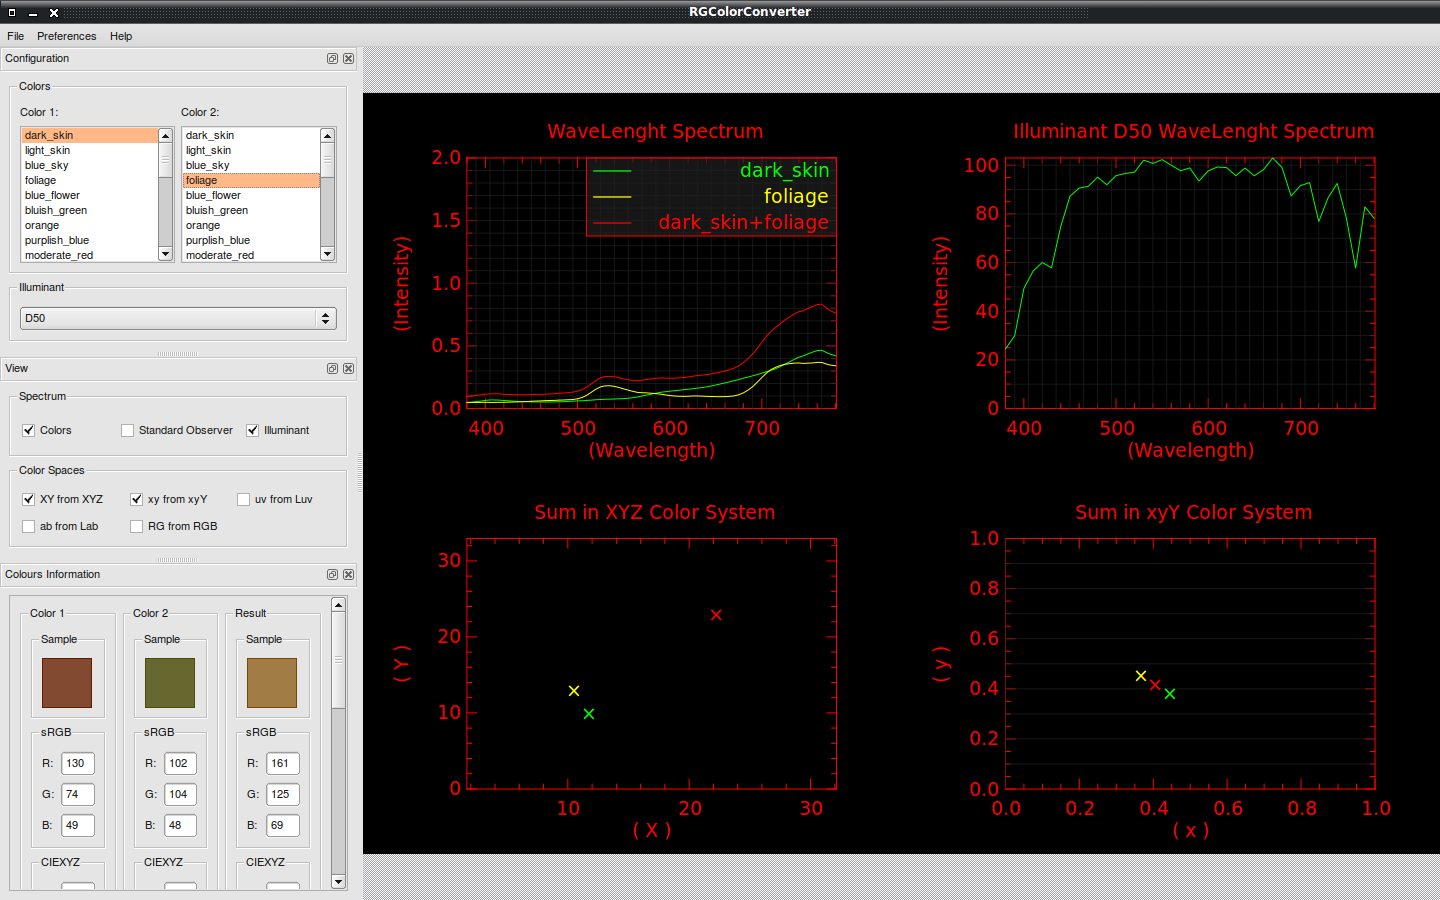
\includegraphics[scale=0.6]
{img/screenshot_RGColorConverter_XYZ_Illuminant_xyY.png}
     \caption{Gráficos do espectro de reflexão das cores iniciais, do
iluminante utilizado (D65) e dos pontos em que as cores se encontram nos
espaços de cor XYZ e L*u*v*.}
     \label{fig:screenshot_XYZ_illuminant_Luv}
\end{figure}

\par
Os dados detalhados da representação das cores em cada um dos espaços de cores
é apresentado na aba "Color Information".

\begin{figure}[!htb]
     \centering
     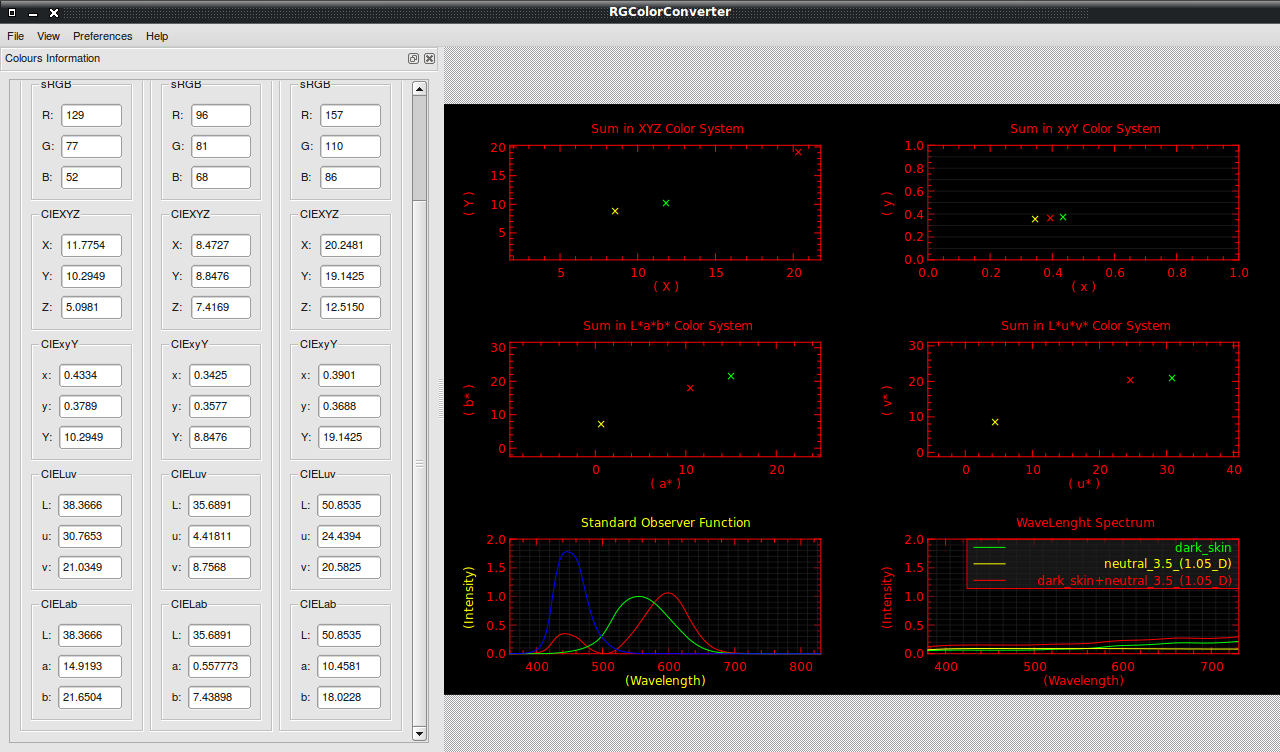
\includegraphics[scale=0.6]{img/screenshot_RGColorConverter_details.png}
     \caption{Resultado da conversão das cores iniciais e da soma dos
espectros em detalhes.}
     \label{fig:screenshot_details}
\end{figure}

\subsection{Instalação}

\subsubsection{Dependências}
\begin{list}{}{}
\item \htmladdnormallink{Qt}{http://qt.nokia.com} (versão 4.6 ou superior)
\item \htmladdnormallink{Plplot}{http://plplot.sourceforge.net/} (versão 5.9.7
ou superior)
\end{list}

\subsubsection{A partir do código-fonte}
\par
Para compilar o código fonte, basta-se ir a raiz da pasta e executar os
sequintes comandos:

\begin{list}{}{}
\item qmake
\item make
\end{list}

\par
Para executar, basta-se executar:
\begin{list}{}{}
\item ./trabCor data/spectral_data_step_5.in
\end{list}

%This repository is for Roberto Azevedo's programs developed in the scope of the
%Foundations of Computer Graphics discipline. This discipline was coursed during
%the Roberto Doctoral course in Pontificial Catholic University of Rio de
%Janeiro
%(PUC-Rio). Marcelo Gattass (http://www.tecgraf.puc-rio.br/~mgattass) was the
%teacher.

%Computer Graphics, PUC-Rio, Color, Image, 3D.

\section{Análise da linearidade dos espaços de cor}
\label{sec:analise_espacos_de_cor}
\par
Esta seção discute a linearidade dos Espaços de Cor apresentados acima, baseado
na implementação do trabalho. Para isso, primeiro temos que definir o que é um
espaço linear.

\par
Um espaço real $R^n$ é dito linear quando, dados:

\begin{equation}\label{eqC1}
C1=(x1,x2, ..., xn)
\end{equation}

\begin{equation}\label{eqC2}
C2=(y1, y2, ..., yn)
\end{equation}

\par
pertencentes a esse espaço, pelo menos as duas propriedades a seguir são válidas
(existem algumas outras propriedades quando o espaço é de número complexos):

\begin{equation}
C_1+C_2 = (x1+y1, x_2+y_2, ..., x_n+y_n); e
\end{equation}
\begin{equation}
\alpha.C_1 = (\alpha.x_1, \alpha.x_2, ..., \alpha.x_n)
\end{equation}

\subsection{CIEXYZ}
\par
Por ser definido como um somatório de operações matemáticas simples (soma e
multiplicação) de um espaço linear (o espaço dos números reais), o espaço de cor
CIE XYZ é naturalmente linear.

\par
A figura a seguir apresenta a soma de duas cores (dark skin e blue sky) no
espaço de cor XYZ. É possível perceber como a soma das duas cores é igual à
soma de cada uma das coordenadas.

\begin{figure}[!htb]
     \centering
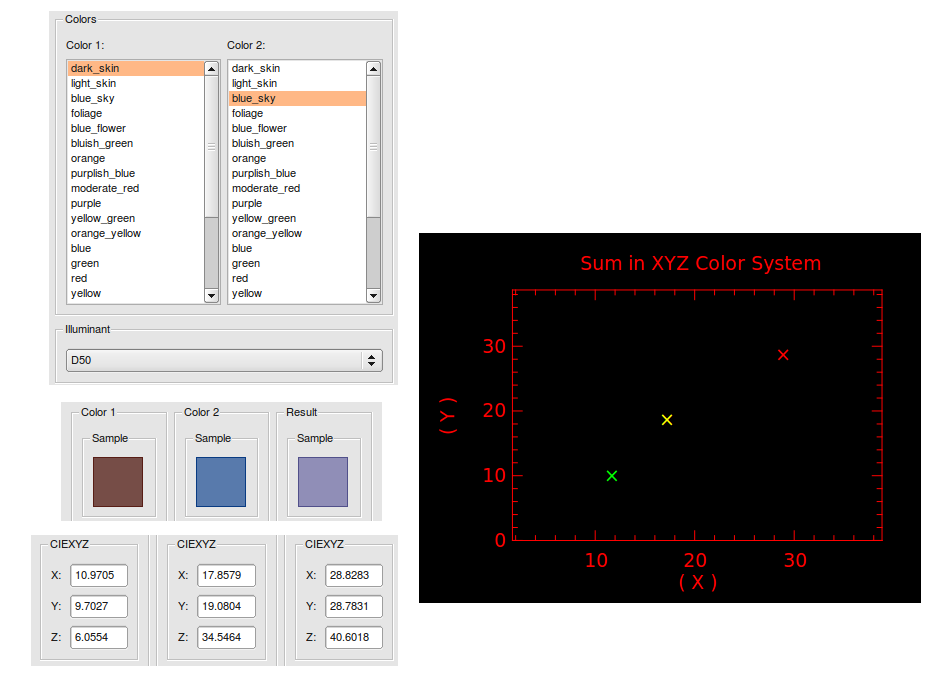
\includegraphics[scale=0.6]{img/XYZ_linearity_sample.png}
     \caption{Resultado da soma de dark skin e blue sky no sistema XYZ.}
     \label{fig:XYZ_linearity_sample}
\end{figure}

\subsection{CIExyY}
As coordenadas de cromaticidade x, y, z são definidas em termos dos valores
dos três estímulos XYZ acima:

\begin{equation}\label{eq:xyz_x}
x=\frac{X}{X+Y+Z}
\end{equation}

\begin{equation}\label{eq:xyz_y}
y=\frac{Y}{X+Y+Z}
\end{equation}

\begin{equation}\label{eq:xyz_z}
x+y+z=1
\end{equation}

\par
Ao somar o espectro de duas cores, o resultado no sistema xyY é uma cor que está
na posição intermediária entre as cores iniciais. Percebe-se assim, claramente
que estamos "misturando" a crominância das duas cores, já que ao traçarmos uma
segmento de reta entre as duas cores originais, esta nova cor estará neste
segmento, com alguma proporção de cada uma das cores originais.

\par
É interessante observar também que ao somarmos os espectros de duas cores
iguais, temos como resultado a mesma cor, mas com uma luminância maior. Por
isso, as componentes de cromaticidade (x e y) são iguais ao valor original e o Y
resultante é um valor maior do que o Y original. A figura a seguir apresenta o
diagrama de cromaticidade xy e onde se encontra a soma de duas cores C1 e C2.

\begin{figure}[!htb]
     \centering
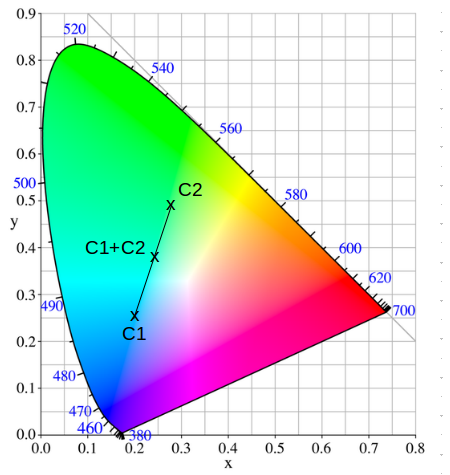
\includegraphics[scale=0.6]{img/xy_linearity.png}
     \caption{Resultado da soma de duas cores no diagrama de cromaticidade xy.}
     \label{fig:XYZ_linearity_sample}
\end{figure}

\par
O sistema xyY não é linear conforme a definição dada acima, já que x e y são
sempre valores entre 0.0 e 1.0. As fórmulas de x e y (vide \ref{eq:xyz_x},
\ref{eq:xyz_y} e \ref{eq:xyz_z}), por normalizarem os valores de XYZ, já dão uma
pista de que nunca poderemos ter uma soma maior que 1.0 em uma das componentes.
Por exemplo, se somarmos 0.8 + 0.8, nunca podemos ter 1.6 como resultado,
invalidando a propriedade I. Contudo, a propriedade que a soma de duas cores
sempre estará na semi-reta entre as duas cores iniciais é bastante útil para
aplicações que manipulam cores.

\subsection{CIELUV (Luv, Lu'v' e L*u*v*)}
\par
O Luv é um espaço de cor proposto na convenção do CIE em 1960. Ele é uma
tentativa de tornar o espaço xyY perceptualmente uniforme, por meio de uma
transformação linear simples. O Luv é definido por:

\begin{equation}\label{eq:Luv_u}
u=\frac{4.X}{X+15.Y+3.Z}=\frac{4.x}{-2.x+12.y+3}
\end{equation}

\begin{equation}\label{eq:Luv_v}
v=\frac{6.Y}{X+15.Y+3.Z}=\frac{6.x}{-2.x+12.y+3}
\end{equation}

\par
Sendo a transformação de uv para xy é dada por:
\begin{equation}\label{eq:Luv_xy}
x=\frac{6.u}{6.u-16.v+12}\;\;\;\; y=\frac{4.v}{6.u-16.v+12}
\end{equation}

\par
Por se tratar de uma transformação linear sobre o xyY, uma reta no espaço xyY 
também se converte em uma reta no espaço Luv. Sendo assim, a mesma linearidade
obtida na soma de duas cores para o xyY é obtida no Luv - ou seja, a soma de
duas cores resulta em um cor que está na semi-reta definida pelas cores
iniciais.

\subsubsection{Lu'v'}
\par
Uma pequena modificação no Luv foi realizada pelo CIE em 1976, definindo um
diagrama de cromaticidade u'v', onde: 

\begin{equation}\label{eq:Lu'v'_u'}
u'=u=\frac{4.X}{X+15.Y+3.Z}=\frac{4.x}{-2.x+12.y+3}
\end{equation}

\begin{equation}\label{eq:Lu'v'_v'}
v'=1.5.v=\frac{9.Y}{X+15.Y+3.Z}=\frac{9.x}{-2.x+12.y+3}
\end{equation}

\par
Mais uma vez, por se tratar de uma simples transformação linear do xyY, a mesma
linearidade se mantém.

\begin{figure}[!htb]
     \centering
     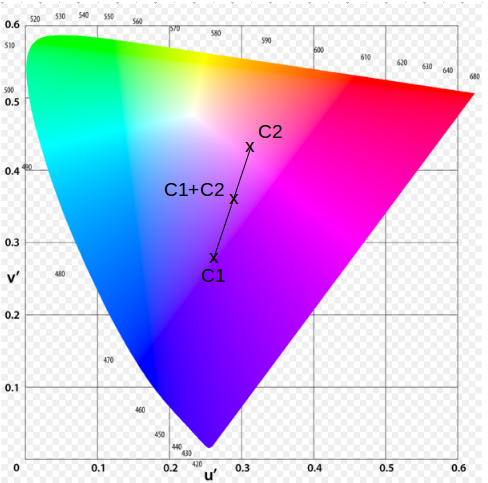
\includegraphics[scale=0.7]{img/luv_linearity.png}
     \caption{Soma de duas cores no diagrama de cromaticidade (u′, v′), também
conhecido como CIE 1976 UCS (uniform chromaticity scale). Fonte: Adaptado de
\htmladdnormallink{Wikipedia}{http://en.wikipedia.org/wiki/CIELUV}}
     \label{fig:cie_1976_luv}
\end{figure}

\subsubsection{L*u*v*}
\par
Contudo, ainda no ano de 1976, também foi proposto pelo CIE o espaço de cor
L*u*v*, sendo este espaço o conhecido como CIELUV. O L*u*v* é definido por:

\begin{equation}\label{eq:L*u*v*_L*}
L^*=116.f(\frac{Y}{Yn})-16,
\end{equation}

\begin{equation}\label{eq:L*u*v*_u*}
u^*=13.L^*.[u'-u_n]
\end{equation}

e

\begin{equation}\label{eq:L*u*v*_v*}
v^*=13.L^*.[v'-v_n]
\end{equation}

\par
Onde $Y_n$ é obtido a partir dos valores dos três estímulos ($X_n$, $Y_n$ e
$Z_n$) para o branco padrão sobre um determinado iluminante (por exemplo, D50
ou D65 que foram utilizados neste trabalho). Da mesma forma, $u_n$ e $v_n$
podem ser obtidos, respectivamente, a partir das formulas \ref{eq:Luv_u} e
\ref{eq:Luv_v}, substituindo-se os valores para os esses três estímulos. E,
$f(s)$ é definida como $f(s) = 7.787.s+16/116$ para valores de $s \le 0.008856$
e $f(s) = s^{1/3}$ para valores de $s > 0.008856$.

\par
No L*u*v*, uma reta no xyY só se converte também em uma reta se o $L^*$ for
constante. A figura a seguir apresenta um exemplo onde uma reta no xyY não se
transforma em uma reta no L*u*v*.

\begin{figure}[!htb]
     \centering
     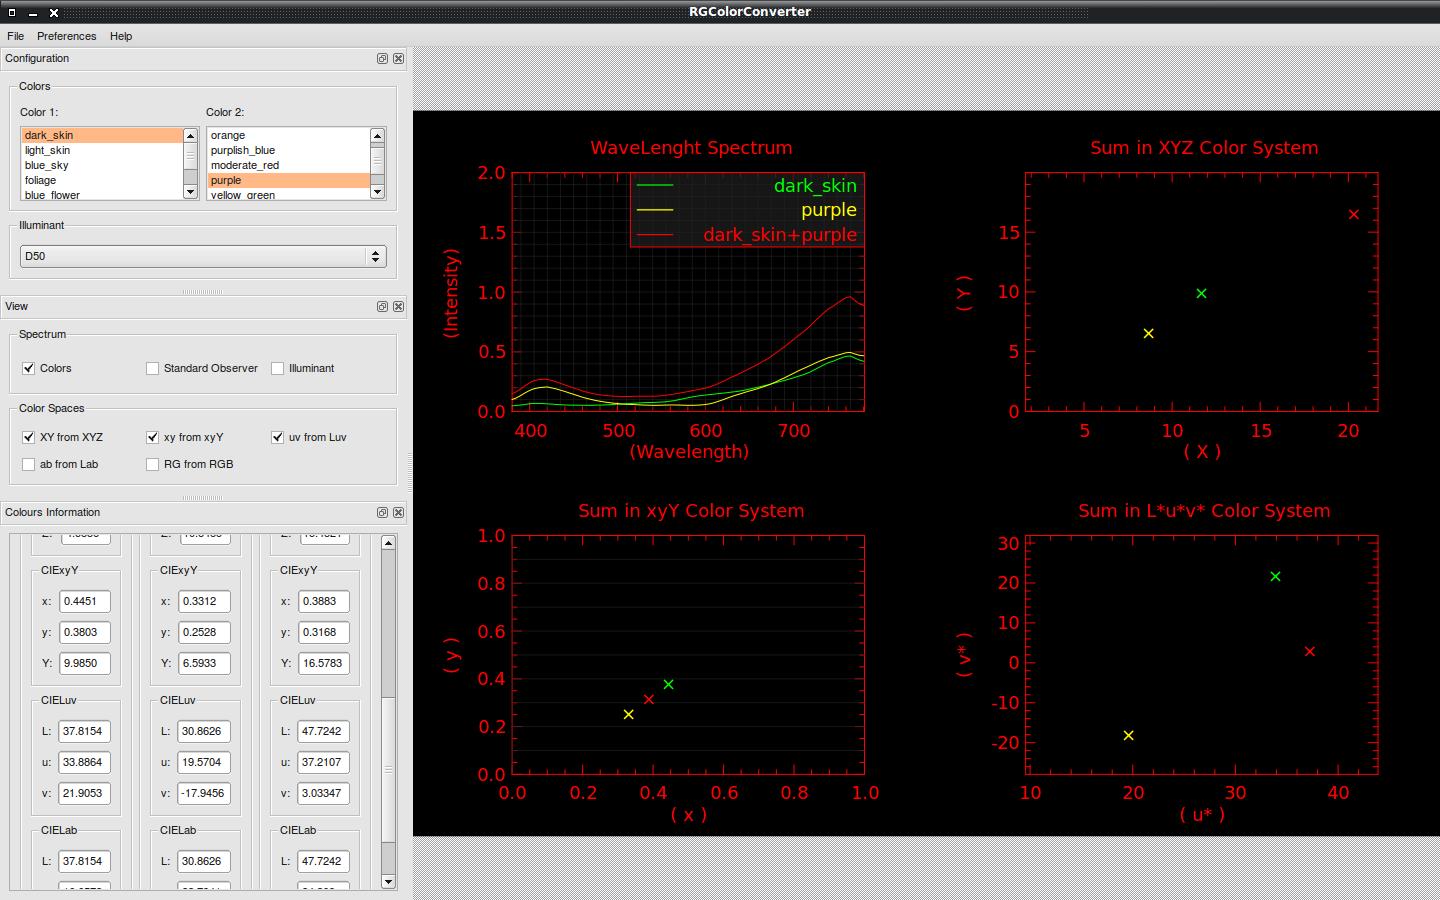
\includegraphics[scale=0.6]{img/luv_no_linearity.png}
     \caption{Exemplo de soma de duas cores (dark_skin e purple) onde uma reta
não se converte em uma reta no diagrama u*v*.}
     \label{fig:luv_no_linearity}
\end{figure}

%TODO: Colocar as figuras comparando Luv, Lu'v' e L*u*v*

\subsection{CIELab}
\par
O espaço de cor CIELab, out CIE $L^* a^* b^*$ foi recomendado na convenção CIE
de 1976. A luminância no espaço CIELab é a mesma definida para o CIELuv,
discutido acima.

\par
Para a conversão do espaço XYZ para o $L^*a^*b^*$ as seguintes fórmulas são
utilizadas:

\begin{equation}\label{eq:L*a*b*_L*}
L^*=116.f(\frac{Y}{Yn})-16,
\end{equation}

\begin{equation}\label{eq:L*a*b*_a*}
a^*=500.\Big[f\Big(\frac{X}{X_n}\Big)-f\Big(\frac{Y}{Y_n}\Big)\Big]
\end{equation}

e

\begin{equation}\label{eq:L*a*b*_b*}
b^*=200.\Big[f\Big(\frac{Y}{Y_n}\Big)-f\Big(\frac{Z}{Z_n}\Big)\Big]
\end{equation}

onde

\[
f(n) = \left\{ 
  \begin{array}{l l}
    t^{1/3} & \quad \text{se} \quad t > \Big(\frac{6}{29}\Big)^3\\
    \frac{1}{3}.\Big(\frac{29}{6}\Big)^2.t+\frac{4}{29} & 
\quad \text{caso contrário}\\
  \end{array} \right.
\]

\par
Quanto a linearidade, uma reta no espaço xyY se transforma em uma curva no
espaço CIELab. O exemplo da Figura a seguir apresenta um exemplo onde uma reta
no diagrama de cromaticidade xy se transforma em uma curva no diagram a*b*.

\begin{figure}[!htb]
     \centering
     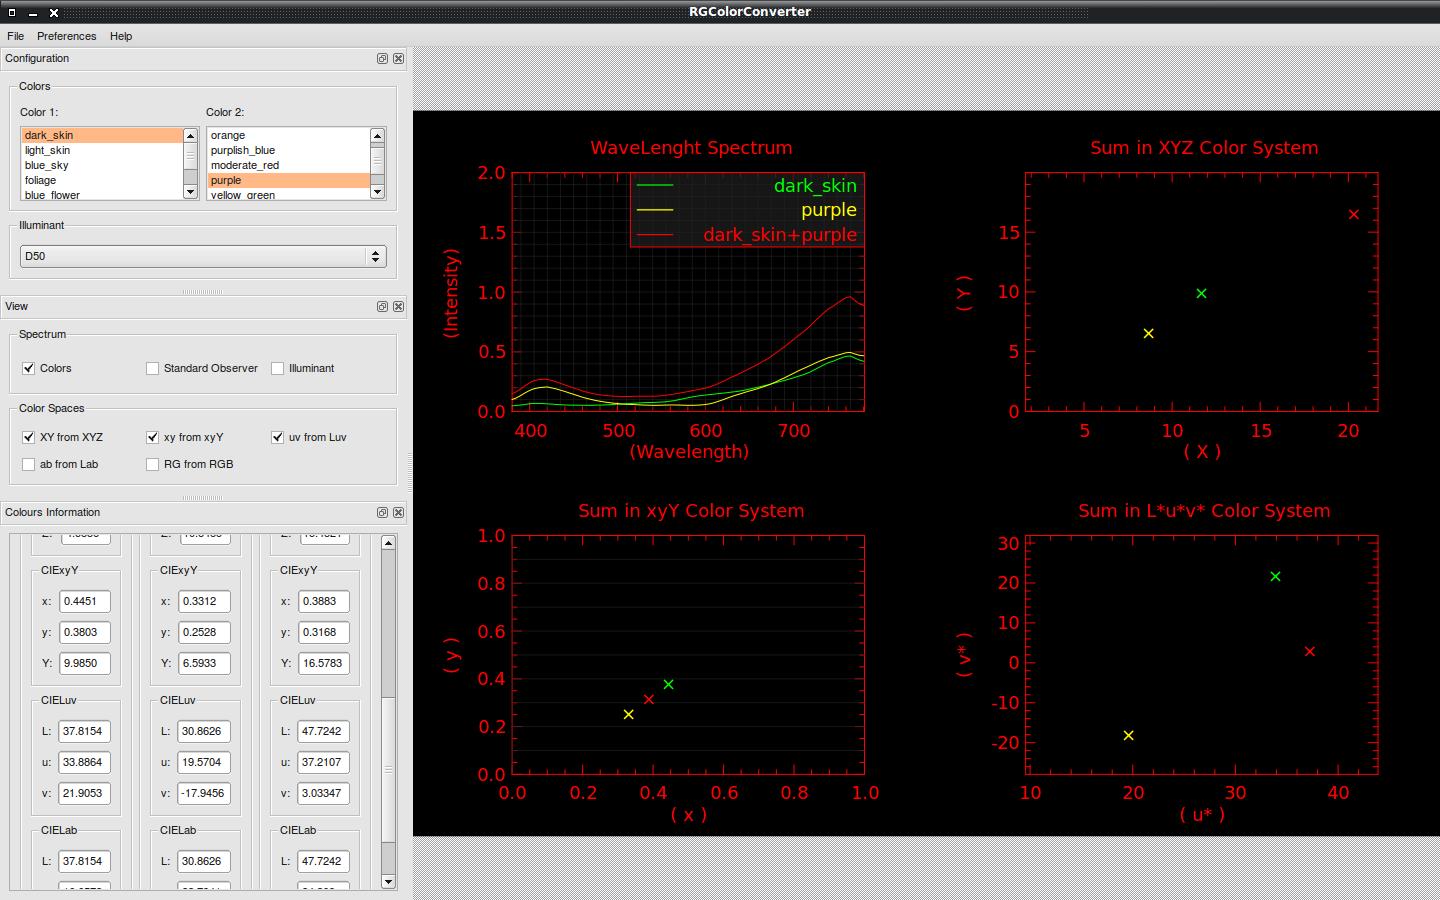
\includegraphics[scale=0.6]{img/luv_no_linearity.png}
     \caption{Exemplo de soma de duas cores (dark_skin e foliage) onde uma reta
no diagrama xy se transforma em uma curva no diagrama a*b*.}
     \label{fig:luv_no_linearity}
\end{figure}

%\subsubsection{Hunter Lab}
%\par
%O espaço de cor Lab foi proposto em 1987 por Hunter e Harols. O Lab surgiu como
%uma tentativa de aproximar o xyY para o modelo perceptualmente uniforme de
%\htmladdnormallink{Munsell}
%{http://pt.wikipedia.org/wiki/Sistema_de_cores_de_Munsell}.

%\par
%Nesse modelo, $L$ representa a luminosidade. O maior valor da luminosidade é
%100, para um branco perfeito. Enquanto $L=0$ representa o preto. O valor de $a$
%representa o quão vermelho (no lado positivo) ou o quão verde (no lado
%positivo) uma cor é. Da mesma similar, o valor de $b$ representa o quão
%amarelado (no lado positivo) ou azulado (no lado negativo) esta cor é. As
%fórmulas a seguir convertem do espaço xyY para o Hunter Lab.

%\begin{equation}\label{eq:Lab_L}
%L^*=100.\Big(\frac{Y}{Y_n}\Big)^{1/2}, 
%\end{equation}

%\begin{equation}\label{eq:Lab_a}
%a=1.785.X_n.\frac{\Big(\frac{X}{X_n}-\frac{Y}{Y_n}\Big)}{\Big(\frac{Y}{Yn}
%\Big)^
%{ 1/2 } }
%\end{equation}

%e

%\begin{equation}\label{eq:Lab_b}
%a=0.5929.Z_n.\frac{\Big(\frac{Y}{Y_n}-\frac{Z}{Z_n}\Big)}{\Big(\frac{Y}{Yn}
%\Big)^{ 1/2 } }
%\end{equation}

\subsection{sRGB}
\par
sRGB é um espaço RGB criado cooperativamente entre a HP e a Microsoft em 1996
para uso em monitores, impressoras e na Internet. As seguintes fórmulas são
utilizadas para o cálculo do sRGB, primeiro calculandos os componentes r, g, b:

\begin{equation}\label{eq:sRGB_r}
r=3.2410.\Big(\frac{X}{X_n}\Big)-1.5374.\Big(\frac{Y}{Y_n}
\Big)-0.4986.\Big(\frac{Z}{Z_n}\Big)
\end{equation}

\begin{equation}\label{eq:sRGB_g}
g=-0.9692.\Big(\frac{X}{X_n}\Big)+1.8760.\Big(\frac{Y}{Y_n}
\Big)-0.0416.\Big(\frac{Z}{Z_n}\Big)
\end{equation}

\begin{equation}\label{eq:sRGB_b}
b=0.0556.\Big(\frac{X}{X_n}\Big)+1.8760.\Big(\frac{Y}{Y_n}
\Big)-1.0570.\Big(\frac{Z}{Z_n}\Big)
\end{equation}

\par
Então, os valores de RGB são calculados como, se $ r < 0.00304 $ como:
$R=12.92.r$, $G=12.92.g$ e $B=12.92.b$. Caso contrário, os valores de R, G e B
sofrem uma correção gama, tal que: $R=1.055.r^\gamma-0.055$,
$G=1.055.g^\gamma-0.055$ e $G=1.055.r^\gamma-0.055$. O valor de $\gamma$
utilizado foi o mais comum: $\frac{1}{2.4}$. Os valores de $X_n$, $Y_n$ e $Z_n$
são calculados para o branco de referência.

\par
É fácil perceber que por não ser uma transformação linear do modelo XYZ, a
linearidade presente no XYZ não se mantém no sRGB. Em especial, também se ao
fator $\gamma$. A Figura a seguir apresenta um exemplo onde é possível
perceber como o sistema sRGB não é linear.

\begin{figure}[!htb]
     \centering
     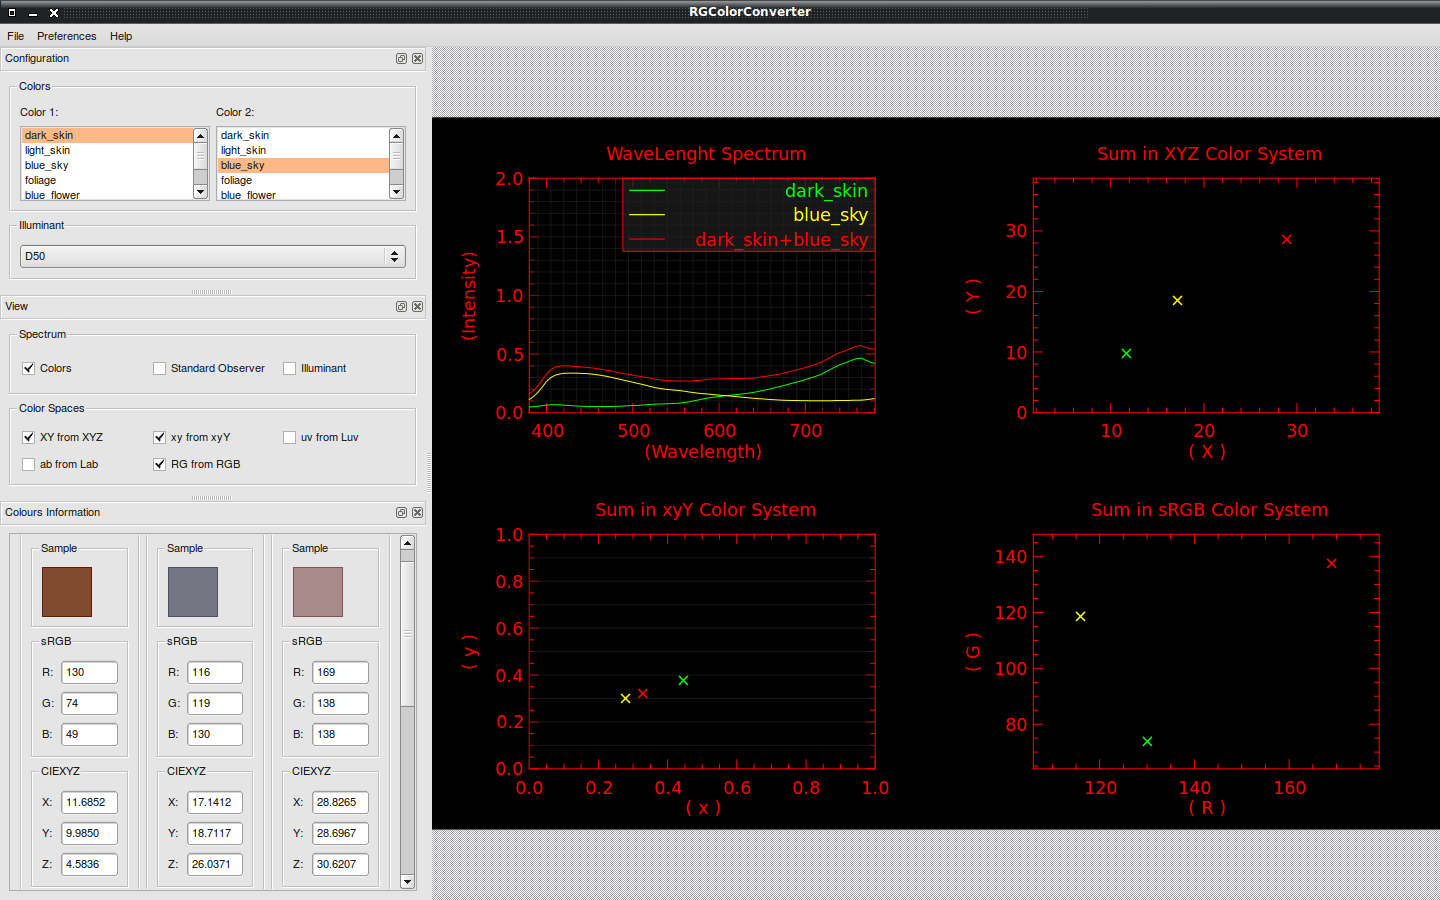
\includegraphics[scale=0.6]{img/srgb_no_linearity.png}
     \caption{Exemplo de soma de duas cores (darkskin e bluesky)
exemplificando a não linearidade do sistema sRGB.}
     \label{fig:luv_no_linearity}
\end{figure}

\section{Trabalhos Futuros}
\par
Entre os trabalhos futuros possíveis encontra-se o mapeamento inteligente para o
gamut de cores, por exemplo, do espaço sRGB. Na implementação atual, caso um
dos valores de R, G ou B sejam encontrados maiores do que 255 ou menores do que
0 eles são simplesmente truncados.

\par
Alguns outros possíveis trabalhos futuros podem ser a transformação de cores
baseada em qual o plano de fundo essa cor irá aparecer. Ou seja, dado a cor em
um background, calcular a cor que deve apresentar sobre esse background
para que a cor original "aparente ser a mesma" quando apresentada sobre este
plano de fundo.

\chapter{Imagem}
Soon.

\chapter{3D}
Soon.

\end{document}
